\begin{Aufgabe}[10]
Hinweis: Alle Teilaufgaben können unabhängig voneinander bearbeitet werden.

\begin{enumerate}
	\item
		Ordnen Sie den Differenzialgleichungen die Richtungsfelder zu:
		
		\begin{tabular}{p{0.25\textwidth}p{0.25\textwidth}p{0.25\textwidth}p{0.25\textwidth}}
			(A) $\displaystyle y' = \frac{x}{y}$ &
			(B) $\displaystyle y' = \frac{y}{x}$ &
			(C) $\displaystyle y' = -\frac{x}{y}$ &
			(D) $\displaystyle y' = -\frac{y}{x}$ \\
		\end{tabular}
		
		\begin{tabular}{llll}
			\ifLoesung
			( {\textcolor{red}C} ) &
			\else
			( \quad ) &
			\fi
			\hspace*{-10mm} \raisebox{-0.8\height}{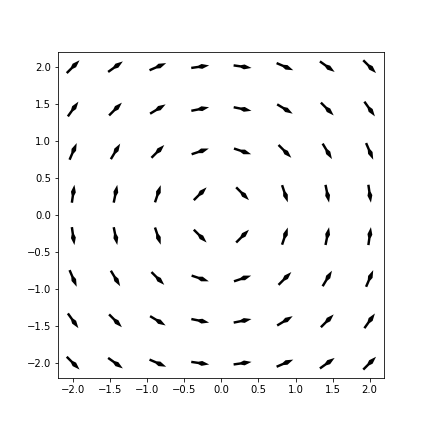
\includegraphics[width=0.4\textwidth]{../M2_IT/m2_it_ws_23_kurzaufgaben_richtungsfeld_3.png}} &
			\ifLoesung
			( {\textcolor{red}D} ) &
			\else
			( \quad ) &
			\fi
			\hspace*{-10mm} \raisebox{-0.8\height}{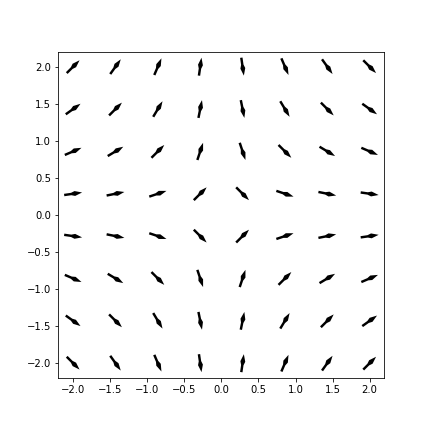
\includegraphics[width=0.4\textwidth]{../M2_IT/m2_it_ws_23_kurzaufgaben_richtungsfeld_4.png}}  \\
			\ifLoesung
			( {\textcolor{red}B} ) &
			\else
			( \quad ) &
			\fi
			\hspace*{-10mm} \raisebox{-0.8\height}{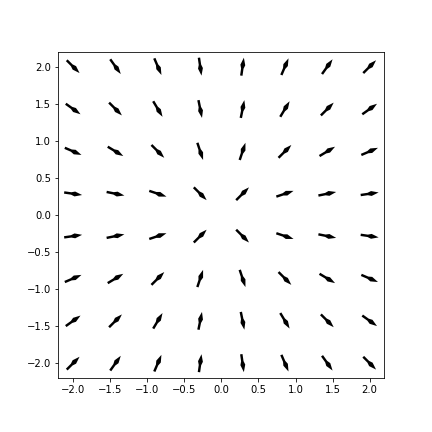
\includegraphics[width=0.4\textwidth]{../M2_IT/m2_it_ws_23_kurzaufgaben_richtungsfeld_2.png}} &
			\ifLoesung
			( {\textcolor{red}A} ) &
			\else
			( \quad ) &
			\fi
			\hspace*{-10mm} \raisebox{-0.8\height}{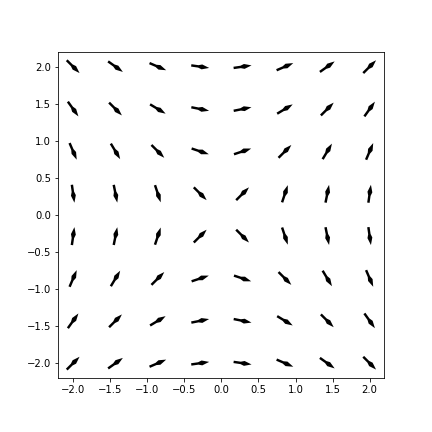
\includegraphics[width=0.4\textwidth]{../M2_IT/m2_it_ws_23_kurzaufgaben_richtungsfeld_1.png}}  \\
		\end{tabular}
		
		\ifLoesung
		\mbox{}\hfill\Punkte{2 P}\\
		\fi	
		
		\pagebreak
	\item
		Bestimmen Sie die allgemeine Lösung der Differenzialgleichung
		\[
			y'(x) = 3 \, x^2 \, y \, .
		\]
		
		\Loesung{10cm}{
			Separation:
			\hfill\Punkte{1 P}
			\[
				\frac{\mathrm{d} \, y}{\mathrm{d} \, x} = 3 \, x^2  \, y 
				\quad \Longrightarrow \quad
				\frac{1}{y} \, \mathrm{d} \, y = 3 \, x^2 \, \mathrm{d} \, x \, .
			\]
			Integration:
			\hfill\Punkte{1 P}
			\[
				\int \frac{1}{y} \, \mathrm{d} \, y = \int 3 \, x^2 \, \mathrm{d} \, x 
				\quad \Longrightarrow \quad
				\ln \left| y \right| = x^3 + C_1, \quad C_1 \in \mathbb{R} \, .
			\]
			Nach $y$ auflösen:
			\hfill\Punkte{1 P}
			\[
				\left| y \right|  = \e^{x^3 + C_1}
				\quad \Longrightarrow \quad
				y = \pm \e^{x^3 + C_1} = \pm \e^C_1 \, \e^{x^3} = C_2 \, \e^{x^3}, \quad C_2 \in \mathbb{R} \, .
			\]
		}
		
	\item
		Berechnen Sie für die Lösung des Anfangswertproblems
		\[
			y'(x) = \frac{y}{1 + x^2}, \quad y(1) = 3 \, ,
		\]
		einen Näherungswert, indem Sie einen Schritt mit dem Euler-Polygonzugverfahren mit der Schrittweite $h=0.2$ durchführen.
		
		\Loesung{}{
			Euler-Polygonzugverfahren:
			\[
			x_1 = x_0 + h = 1.2, 
			\quad
			\tilde{y}_1 = 
			\tilde{y}_0 + h \cdot  \frac{\tilde{y}_0 }{1 + x_0^2} = 
			3 + 0.2 \cdot  \frac{3}{1 + 1^2} = 3.3 \, .
			\hfill\Punkte{2 P}
			\]
		}
		
		\newpage
		
	\item
		Beurteilen Sie den folgenden Dialog mit ChatGPT 3.5.
		Sind die Berechnungen und die Behauptungen von ChatGPT korrekt?
		 
		 \vspace*{2ex}
		 
		 \textbf{You}
		 
		Bitte erstelle ein Beispiel für ein lineares Differenzengleichungssystem mit zwei Unbekannten, das asymptotisch stabil ist.
		
		\vspace*{2ex}
		
		\textbf{ChatGPT}
		
		Betrachten wir das folgende lineare Differenzengleichungssystem mit zwei Unbekannten:
		\[
			\begin{array}{lcl}
				x_{k+1} & = & 0.8 \, x_k + 0.2 \, y_k \\
				y_{k+1} & = & 0.4 \, x_k + 0.6 \, y_k
			\end{array}
		\]
		Die obigen Gleichungen können in Matrixform geschrieben werden als:
		\[
			\left(
				\begin{array}{c}
					x_{k+1} \\
					y_{k+1}
				\end{array}
			\right)
			= 
			\left(
			\begin{array}{cc}
				0.8 & 0.2 \\
				0.4 & 0.6
			\end{array}
			\right)
			\left(
			\begin{array}{c}
				x_{k} \\
				y_{k}
			\end{array}
			\right), \mbox{ mit der Matrix }
			\mathbf{A} =
			\left(
			\begin{array}{cc}
				0.8 & 0.2 \\
				0.4 & 0.6
			\end{array}
			\right)
		\]
		Die Matrix $\mathbf{A}$ ist die Übertragungsmatrix des Systems.
		Um die asymptotische Stabilität zu überprüfen, betrachten wir die Eigenwerte dieser Matrix.
		Die Eigenwerte $\lambda$ können durch das Lösen der charakteristischen Gleichung gefunden werden:
		\[
			\left|
				\begin{array}{cc}
					0.8 - \lambda & 0.2 \\ 
					0.4 & 0.6 - \lambda
				\end{array}
			\right| = 0
			\quad \Longleftrightarrow \quad
			(0.8 - \lambda)(0.6 - \lambda) -0.2 \cdot 0.4 = 0
			\quad \Longleftrightarrow \quad
			\lambda^2 - 1.4 \, \lambda + 0.4 = 0
		\]
		Die Lösungen dieser quadratischen Gleichung sind $\lambda_1=1$ und $\lambda_2=0.4$.
		Beide Eigenwerte haben Beträge kleiner als $1$, was darauf hinweist, dass  das System asymptotisch stabil ist.
		In diesem Beispiel konvergieren die Lösungen für $x_k$ und $y_k$ gegen Null, was auf eine asymptotische Stabilität hinweist.  
		
		\Loesung{}{
			Die Berechnungen sind korrekt.
			Das System ist jedoch nicht asymptotisch stabil, denn der Betrag des Eigenwerts $\lambda_1 = 1$ ist nicht echt kleiner $1$.
			Deshalb konvergieren auch nicht alle Lösungen gegen Null.
			Beispielsweise ist $x_0=1$ und $y_0=1$ ein Fixpunkt. 
			\hfill\Punkte{3 P}
		}
			
	\end{enumerate}
	
\end{Aufgabe}

\newpage

\endinput